\documentclass{article}

\usepackage{amsmath}
\usepackage[brazil]{babel}
\usepackage[utf8]{inputenc}
\usepackage{graphicx}
\usepackage{geometry}
\usepackage{url,color}

\geometry{a4paper, top=2cm, left=2cm, right=2cm, bottom=2.7cm}

\title{Implementação filtro média móvel em VHDL}

\date{\today}

\begin{document}

\maketitle

\section{Média móvel com quatro coeficientes}

Implementação baseada em \cite{ped} e arquivos de audio gerados em \cite{oce}.

\subsection{Diagrama}

\begin{figure}[!htb]
	\centering
	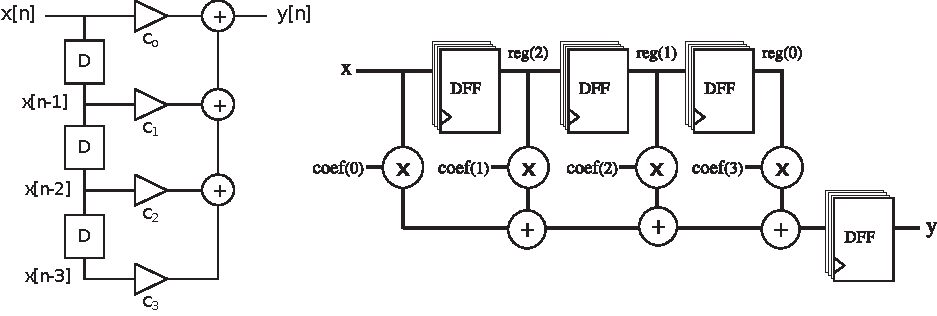
\includegraphics[scale=1]{fir.pdf}
	\caption{Diagrama e RTL do filtro FIR}
	\label{fig:fir}
\end{figure}

\subsection{Equação}

\begin{eqnarray}
	y[n] = \sum_{k=0}^{M}c_kx[n-k]
\end{eqnarray}

\subsection{Exemplo de arquivo de entrada}

\begin{verbatim}
(hex) 00  34  EF 67  16 38 53  F0 4B  E1   EF  FF  9A  FF  A6  CE (...)
(dec) 0   52 -17 103 22 56 83 -16 75 -31  -17 -1  -102 -1 -60 -50
\end{verbatim}


\subsection{Todos os coeficientes = 1, dividindo por 4 no final}

\begin{eqnarray}
	y[0] &=& c[0] . x[0] = 52 . 1 = 52/4 = 13 \nonumber \\
	y[1] &=& c[0] . x[1] + c[1] . x[0] = -17 + 52 = 35 / 4 = 8 \nonumber \\
	y[2] &=& c[0] . x[2] + c[1] . x[1] + c2 . x[0] = 103 - 17 + 52 = 138/4 = 34 \nonumber \\
	y[3] &=& c[0] . x[3] + c[1] . x[2] + c2 . x[1] + c3 . x[0] = 22 + 103 - 17 + 52 = 160/4 = 40 \nonumber \\
	y[4] &=& c[0] . x[4] + c[1] . x[3] + c2 . x[3] + c3 . x[1] = 56 + 22 + 103 - 17 = 164/4 = 41 \nonumber \\
	y[5] &=& \dots \nonumber
\end{eqnarray}

\subsection{Exemplo de arquivo de saída}

\begin{verbatim}
(hex) 00 0D 08 22 28 29 42 24 31 1B 02 06 DA E1 (...)
(dec) 00 13  8 34 40 41 66 36 49 27 2 6 -38 -31 (...)
\end{verbatim}

\subsection{Fonte de audio teste440\_2000 (tom em 440Hz e 2000Hz)}

\begin{figure}[!htb]
	\centering
	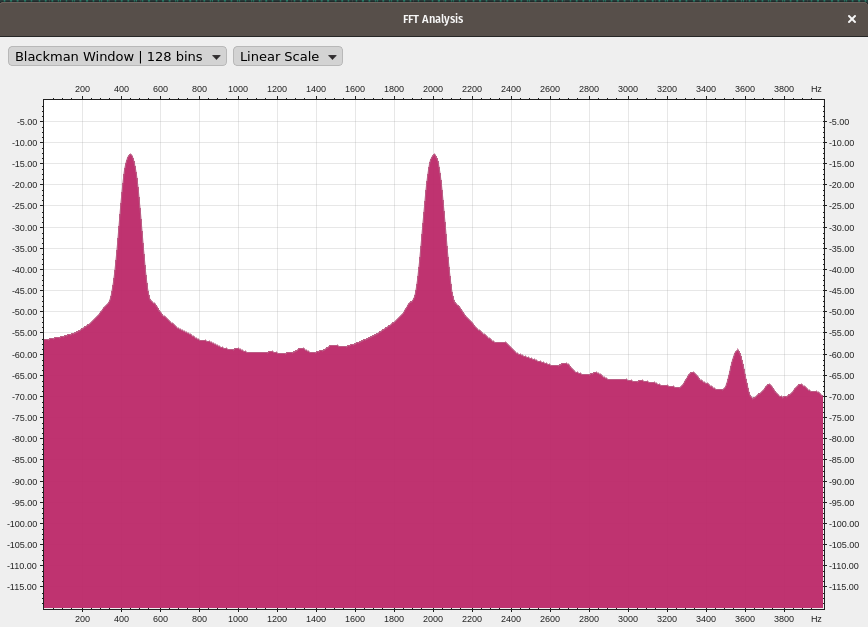
\includegraphics[scale=1]{teste440_2000.png}
	\caption{Sinal de entrada: 440 e 2000Hz.}
	\label{fig:fir1}
\end{figure}

\begin{figure}[!htb]
	\centering
	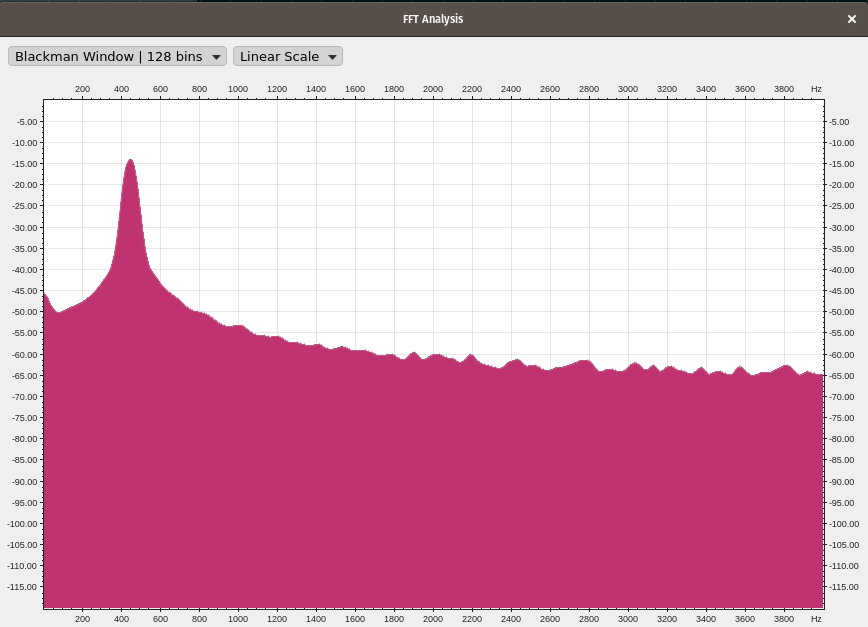
\includegraphics[scale=1]{saida_teste440_2000.png}
	\caption{Saída pós filtro.}
	\label{fig:fir2}
\end{figure}



\begin{thebibliography}{9}
	\bibitem[1]{ped} Pedroni, Volnei A. \textbf{Circuit design with VHDL}. MIT Press, 2004.

	\bibitem[2]{oce} Ocenaudio. \url{https://www.ocenaudio.com/}
\end{thebibliography}


\end{document}
